\documentclass[sigconf,anonymous,review]{acmart}

\usepackage{booktabs}
\usepackage{makecell}
\usepackage{algorithm}
\usepackage[noend]{algpseudocode}
\usepackage{array}
\usepackage{multirow}
\usepackage{float}
\emergencystretch=3em

\settopmatter{printacmref=false}
\setcopyright{none}
\renewcommand\footnotetextcopyrightpermission[1]{}
\acmConference[WWW '27]{The ACM Web Conference 2027}{2027}{TBD}
\acmYear{2027}
\acmDOI{}
\acmISBN{}

% Single definition of the anonymous artifact link (placeholder until the anonymous mirror is created).
\providecommand{\anonrepo}{\url{https://anonymous.4open.science/r/freeze-then-certify-ANON}}

\newcommand{\cA}{\mathcal{A}}
\newcommand{\eps}{\varepsilon}
\newcommand{\dmain}{\delta_{\text{main}}}
\newcommand{\dvar}{\delta_{\text{var}}}
\newcommand{\Npen}{N_{80}^{\text{pen}}}
\newcommand{\meff}{m_{\text{eff}}}
\AtEndPreamble{\theoremstyle{acmdefinition}\newtheorem{remark}[theorem]{Remark}}

\begin{document}

\title{Freeze, Then Certify: Finite-Population Joint Certificates for Budgeted Targeting Policies on Randomized Logs}

\author{Anonymous Author(s)}
\affiliation{%
  \institution{Anonymous Institution}
  \country{}}

\begin{abstract}
A platform choosing budget-constrained targeting policies from a randomized log may want a finite-sample guarantee that, at every budget at once, its choice is near-optimal for the value a full analysis of the logged table would compute, paid for in outcome reads. Freezing the read plan lets one finite-population Chernoff width per policy difference keep all certificates on a 15-budget frontier simultaneously valid. It certifies 12 of the 15 problems with 0.30--0.82 times the outcome reads of matched-strength per-cell rectangles on two reused logs and a never-replayed one. Our certificate, FDC-BF, bounds each segment-arm cell with a Bennett inequality carrying the exact finite-population variance and sums these bounds along each policy difference under one union ledger. Its probability of any false certificate is at most $\delta = 0.05$, also under monitoring at any time on its frozen schedule. At matched time-uniform strength, FDC-BF needed 0.71 and 0.53 times the reads of a betting rectangle and of a rectangle with its own cell bound on Criteo (one-sided 95\% bounds 0.723, 0.542), and 0.37 and 0.30 times on X5 RetailHero (0.379, 0.308). A knapsack program, FDC-DP, evaluates this certificate family on classes too large to list. With 16--64 segments and rule-selected tolerances at which most feasible policies are $\eps$-optimal, it needed 0.17--0.63 times the reads of the matched time-uniform rectangle on X5 and Lenta. On the never-replayed Open Bandit Dataset with traffic-share costs, it needed 0.817 times them (bound 0.824, preregistered threshold 0.90). Bounds describe replay variation within each log.
\end{abstract}

\begin{CCSXML}
<ccs2012>
 <concept>
  <concept_id>10002950.10003648.10003662.10003666</concept_id>
  <concept_desc>Mathematics of computing~Hypothesis testing and confidence interval computation</concept_desc>
  <concept_significance>500</concept_significance>
 </concept>
 <concept>
  <concept_id>10002951.10003260.10003272</concept_id>
  <concept_desc>Information systems~Online advertising</concept_desc>
  <concept_significance>300</concept_significance>
 </concept>
</ccs2012>
\end{CCSXML}
\ccsdesc[500]{Mathematics of computing~Hypothesis testing and confidence interval computation}
\ccsdesc[300]{Information systems~Online advertising}

\keywords{policy certification, budgeted targeting, sampling without replacement, finite-sample guarantees, outcome-access cost, uplift, preregistration}

\maketitle

%% =====================================================================
\section{Introduction}\label{sec:intro}

A platform that has run a randomized targeting experiment must choose which budget-constrained policy to deploy and, if it wants to bound the risk of that decision, as experimentation platforms do for ship decisions~\citep{schultzberg2024riskaware}, needs an error guarantee rather than a point ranking. Budgeted targeting from experiment data is industrial practice~\citep{zhao2019uplift,ai2022lbcf}, and the treated fraction may be recalibrated after deployment, as Booking.com does online for ROI-constrained promotions~\citep{goldenberg2020freelunch}, so the guarantee should hold at every budget on the frontier at once. With probability at least $1-\delta$, each chosen policy should be within $\eps$ of the best feasible one, in the spirit of always-valid experiment reports~\citep{johari2017peeking,howard2021time}. This is a question of decision sufficiency relative to the logged table: a certificate says the chosen policies are those a full analysis of every logged outcome would rank near-best, not that they are optimal for future users (\S\ref{sec:setting}). We count its cost in logged outcomes revealed to the certifier, which binds when outcome access is priced per record (\S\ref{sec:setting}). The paper therefore asks how few logged outcomes a frontier-wide finite-sample guarantee needs.

Direction-level certificates already exist, and so does their validity under a fixed design. RAGE~\citep{fiez2019sequential}, Peace~\citep{katzsamuels2020empirical}, static allocations~\citep{soare2014best} and likelihood-ratio stopping~\citep{garivier2016optimal,jourdan2021efficient} bound each policy difference with one width, with thresholds proven for sampling with replacement. For a sample of fixed size, Hoeffding's convex-order theorem~\citep{hoeffding1963probability} carries fixed-design moment-generating-function bounds over to sampling without replacement, so a frozen design inherits thresholds built from them. The time-uniform without-replacement sequences used to audit finite pools~\citep{waudbysmith2020confidence,waudbysmith2024estimating} work per (segment, arm) cell instead. Added along a policy difference as a sum of radii, they form a \emph{rectangle}, which charges a worst-case radius in every cell even when cell errors partly cancel. The open question is how much a finite-population joint width saves over such rectangles, and what keeps it valid frontier-wide and at any monitoring time.

Freezing the read plan lets one finite-population Chernoff width per policy difference keep the whole frontier's certificates simultaneously valid and certify 12 of 15 problems with 0.30--0.82 times the outcome reads of matched-strength per-cell rectangles on two reused logs and a never-replayed one. With the plan fixed, each cell at each checkpoint is a uniform without-replacement sample of known size. Its moment generating function then has a Bennett bound with the \emph{exact} finite-population variance. Summed along a policy difference, these bounds give one width that grows like the $\ell_2$ norm of the cell errors, whereas a rectangle grows like their $\ell_1$ sum. Beyond Hoeffding's transfer, we combine this finite-population lemma with exact variance boxes, a union ledger over the budget frontier, a time-uniform extension and a proposition that predicts when the joint width wins. The ledger and the extension apply standard tools, a union bound and reverse martingales; FDC-DP, a knapsack dynamic program, evaluates the certificate on classes too large to list (\S\ref{sec:validity}, \S\ref{sec:scale}).

FDC-BF (Figure~\ref{fig:method}) implements this argument on a balanced 50/50 plan, with one ledger over (problem, feasible policy, checkpoint) (Theorem~\ref{thm:fdcbet}). A reverse-martingale argument extends it to monitoring at any time (Remark~\ref{rem:tu}). Proposition~\ref{prop:width} splits its width ratio against a rectangle with the same cell bound into a union cost and an aggregation gain, so the saving grows with the effective number of cells carrying a policy difference's error.

\begin{figure}[t]
\centering
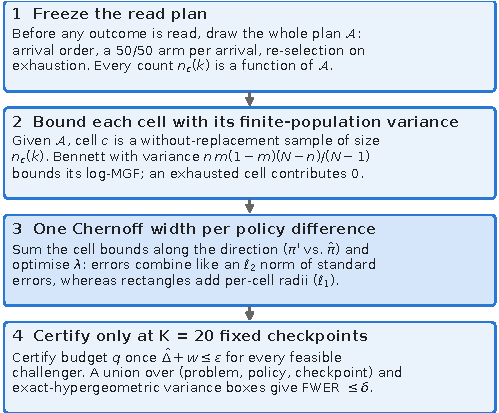
\includegraphics[width=0.72\columnwidth]{figures/fig1_fdcbf.pdf}
\caption{\textbf{FDC-BF in four steps.} Steps 1, 3 and 4 are shared with its Bernstein variant (App.~\ref{app:proofs}); step 2, the finite-population cell bound, defines FDC-BF. No rectangle does step 3. Only step 1 restricts how rows are read.}
\label{fig:method}
\Description{Four stacked boxes connected by arrows: freeze the read plan; bound each cell with its finite-population variance; one Chernoff width per policy difference; certify only at 20 fixed checkpoints.}
\end{figure}

The evidence comes from preregistered tests on fresh replay randomizations of two real logs, Criteo and X5 RetailHero. In the headline \emph{time-uniform test}, every method is monitored at the same 77 times. On Criteo, FDC-BF then reaches 12 of 15 certified budget problems at 0.87M rows against 1.23M for the betting rectangle and 1.64M for the matched rectangle, which shares its cell bound. On X5 it needs 23.7k rows against 63.4k and 78.0k. These geometric means over 200 paired streams hold for the registered rivals on these two reused tables. Two earlier preregistered tests at checkpoint strength gave ratios of 0.64--0.66 on Criteo and 0.36 on X5, so the ordering holds at both guarantee strengths. A last test replays a log that no earlier test had touched, the Open Bandit Dataset~\citep{saito2021open}, where the knapsack form FDC-DP needed 0.817 times the reads of the matched time-uniform rectangle, so the saving survives outside the reused tables.

Several choices, FDC-BF itself among them, came after earlier evaluations (\S\ref{sec:deviations}). With this stated, we make four claims, each with a falsification condition.

\begin{itemize}
\item[\textbf{C1}] \textbf{Validity.} For every frozen plan, FDC-BF falsely certifies any of 15 budget problems at any of 20 checkpoints with probability at most $\delta = 0.05$. The bound also holds for certification at any later time with widths frozen at the last checkpoint, and for FDC-DP, which evaluates the same certificate family on one global $\lambda$ grid per checkpoint without listing the class. Its core is the exact-variance Bennett lemma (Lemma~\ref{lem:bennett}), a finite-population moment bound for each frozen cell. \emph{Falsified by} a flaw in the proofs (\S\ref{sec:validity}, App.~\ref{app:proofs}); replay can reveal only gross violations.
\item[\textbf{C2}] \textbf{Fewer reads than rectangles (confirmatory, four logs).} At matched time-uniform strength, the one-sided 95\% bound on FDC-BF's paired geometric-mean $\Npen$ ratio is below 0.85 (Criteo) and 0.50 (X5) against each of the two registered time-uniform rectangles. At checkpoint strength it is below 0.80 and 0.60 against each registered rectangle, and no FDC-BF stream is false. With 16 to 64 segments, at development-rule-selected tolerances, FDC-DP's bound against the matched time-uniform rectangle is below 0.80 in each of five cells on X5 and Lenta, and below 0.90 on the never-replayed Open Bandit Dataset with traffic-share knapsack costs. \emph{Falsified by} a bound at or above its threshold or by any false stream (Tables~\ref{tab:main} and~\ref{tab:scale}, \S\ref{sec:obd}).
\item[\textbf{C3}] \textbf{An informed frozen plan beats the tested adaptive designs (post hoc, semi-synthetic).} At equal pilot information, frozen pilot-Neyman FDC-BF has a smaller paired geometric-mean $\Npen$ than each tested reset and menu adaptive joint certificate in four constructed regimes, also with the pilot charged to both. Against adaptive designs without a pilot, charging it to the frozen plan alone reverses this on X5-sized tables unless several runs share it. \emph{Falsified by} an equal-information ratio whose 95\% interval reaches 1 (\S\ref{sec:c3}, supplement S11).
\item[\textbf{C4}] \textbf{Mechanism (descriptive).} With the same cell bound, boxes, $\delta$ split and plan, the joint width needs about half (Criteo) and under a third (X5) of the rectangle's rows at either strength. The log with more effective cells gains more, and a tighter cell bound changes little. \emph{Falsified by} a matched ratio above 0.8, a log ordering opposite to the effective-cell ordering, or a cell-bound ablation that saves more than aggregation (\S\ref{sec:c4}).
\end{itemize}

\noindent Our contributions map onto these claims: the finite-population joint certificate with its frontier ledger and time-uniform extension (C1), the width proposition (C4) and the preregistered and post-hoc evidence (C2, C3). FDC-DP, a knapsack evaluation of the same certificate family on a global $\lambda$ grid, extends C1 and C2 to implicit policy classes and to a log whose evaluation outcomes informed no design choice. Code, locks, seeds and seals are in the anonymous repository (\anonrepo). Section~\ref{sec:setting} first fixes what is certified, so that no method can gain speed by certifying something weaker.

%% =====================================================================
\section{Problem Setting}\label{sec:setting}

This section fixes the target: $\eps$-optimal answers to $Q$ budget problems on the logged finite population, held simultaneously with probability at least $1-\delta$ during a without-replacement replay.

\textbf{Log, cells and estimand.} Everything certified is a function of one fixed table. The evaluation half of a randomized log is split into $S$ segments and $A$ arms. Each cell $c = (s,a)$ holds a finite pool of $N_c$ binary outcomes with pool mean $\mu_c$. Segment weights are $w_s = \sum_a N_{s,a}/\tau_R$, where $\tau_R$ is the number of rows in the half. On Criteo (CR9), $S = 9$, $A = 2$ and $\tau_R = 6{,}989{,}799$; on X5 (X9), $S = 9$, $A = 2$ and $\tau_R = 100{,}393$. The estimand is the observed-pool policy value of this table, the stratified value an analyst reading every outcome of the half would compute. The certificate controls only the error of reading part of the table: it does not control randomness in treatment assignment or the counterfactual outcomes missing from each pool, even for the logged users, so it does not bound causal deployment regret.

\textbf{Policies and budget problems.} The objects to certify are the best budget-feasible policies. A policy $\pi \in [A]^S$ assigns an arm to each segment, with value $J(\pi) = \sum_s w_s \mu_{s,\pi(s)}$ and cost $C(\pi) = \sum_s w_s \mathbb{1}[\pi(s) = 1]$, the treated fraction. Problem $q$ has budget $B_q$, feasible class $\Pi_{B_q} = \{\pi : C(\pi) \le B_q\}$ and optimum $\pi^*_q$. We use $Q = 15$ budgets $B_q \in \{0.10, 0.15, \dots, 0.80\}$. On Criteo the classes hold 14 to 443 of the 512 policies, $\sum_q |\Pi_{B_q}| = 3{,}386$ on both logs, and every class is enumerated exactly. Because the classes are large and overlap, one $\delta$ over the whole frontier is the relevant guarantee.

\textbf{Replay, checkpoints and endpoint.} Speed is measured in logical rows read. A replay stream fixes a uniformly random arrival order of segments and a uniformly random order of records inside each pool. At each arrival a method chooses which arm's pool to read next. Under the checkpoint protocol, certificates are issued only at $K = 20$ checkpoints, log-spaced from 50,000 rows on Criteo (2,000 on X5) to $\tau_R$, so consecutive checkpoints differ by a factor of 1.297 on Criteo and 1.229 on X5. The primary endpoint $N_{80}$ is the first checkpoint at which at least 12 of 15 problems are certified. $\Npen$ sets it to $\tau_R$ if a false certificate occurs or 12 of 15 is never reached. We report logical reads, not I/O savings.

\textbf{When outcome reads are the binding cost.} The frozen plan needs each row's segment and arm, never its outcome; if outcomes are stored and free, a full scan needs no certificate. Reads dominate when each outcome read is billed, as in clean rooms that bill record matching per record, e.g.\ AWS at \$0.50 per 1,000 records matched~\citep{awscleanrooms2026pricing}; under individual privacy accounting, which can make leaving outcomes unaccessed valuable~\citep{ebadi2015personal,feldman2021individual}; and when outcomes are labelled per item, e.g.\ a SageMaker Ground Truth fee of \$0.04 per object (50k--1M tier, labour excluded)~\citep{awssagemaker2026pricing}, or delayed~\citep{chapelle2014modeling}. Reads also proxy experiment size: platforms use anytime-valid tests so that an experiment can stop once its evidence suffices~\citep{johari2017peeking,lindon2026anytime,schultzberg2023sequential}. A 50/50 replay is not a prefix of the original logging order, so fewer replay reads correspond only approximately to a smaller or shorter experiment, and $N_{80}$ counts outcomes revealed, not users enrolled. FDC-BF is not differentially private. The target fits a decision that would otherwise be made by analysing every logged outcome, such as choosing the budgeted rules a full-log uplift analysis would pick; it says nothing about future users.

\textbf{Guarantee.} A certificate for problem $q$ at checkpoint $k$ freezes an answer $\hat\pi_q$ and is false if $J(\pi^*_q) - J(\hat\pi_q) > \eps$. We use $\eps = 0.001$ on Criteo's visit rate (mean 0.047) and $\eps = 0.02$ on X5's purchase rate (development mean about 0.62). A method is valid if the probability that a stream contains any false certificate, over all problems and checkpoints, is at most $\delta = 0.05$. Every compared guaranteed method must prove this, and \S\ref{sec:method} now builds one that does.

%% =====================================================================
\section{FDC-BF: Freeze, Then Certify Jointly}\label{sec:method}

This section builds the certificate in the four steps of Figure~\ref{fig:method}; the proof in \S\ref{sec:validity} needs each of them.

\textbf{Step 1: frozen balanced plan.} The read plan contains no outcome information by construction. Before any outcome is read, FDC-BF fixes the complete plan $\cA$: the segment arrival order, a planned arm per arrival with probability 1/2 each, and a uniform variable per arrival for re-selection when a planned pool is exhausted. Exhaustion depends only on counts and pool sizes, so the count $n_c(k)$ of rows read from cell $c$ by checkpoint $k$ is a function of $\cA$, which must be independent of the within-pool record order. Balance suits the problem: each policy difference contrasts two arms of a segment with equal weight and the arms' standard deviations on Criteo are close (0.192 and 0.215), whereas the log's 85/15 split starves control cells.

\textbf{Step 2: a finite-population bound for each cell.} Conditional on $\cA$, cell $c$ at checkpoint $k$ is a uniform without-replacement sample of size $n = n_c(k)$ from a pool of $N = N_c$ binary outcomes with mean $m = \mu_c$, and the cells are independent. The hypergeometric count has a probability generating function with only real roots. It therefore has the law of a sum of $n$ independent Bernoulli variables whose variances add up to the exact finite-population variance~\citep{vatutin1982limit,tang2023poisson}. Bennett's lemma~\citep{bennett1962probability} applied to each summand gives, for every real $u$,
\begin{equation}\label{eq:cell}
\begin{gathered}
\log \mathbb{E}\, e^{u(\hat\mu_c - m)} \le \Psi_c(u; m) := n\, m(1-m)\,\frac{N-n}{N-1}\,\phi\!\left(\frac{|u|}{n}\right),\\
\phi(x) = e^x - 1 - x,
\end{gathered}
\end{equation}
with $\Psi_c = 0$ for an exhausted cell. Its Bernstein variant, built on Hoeffding's comparison~\citep{hoeffding1963probability}, lacks the factor $(N-n)/(N-1)$. It matters on a balanced plan: at FDC-BF's typical stopping point of 0.13\,$\tau_R$ rows on Criteo, about 43\% of a control pool is read.

\textbf{Step 3: one Chernoff width per policy difference.} For a challenger $\pi'$ and a centre $\hat\pi$, the estimation error of their difference is linear in the cell errors: $Y = \sum_c a_c(\hat\mu_c - \mu_c) = \Delta(\pi',\hat\pi) - \hat\Delta(\pi',\hat\pi)$. Here $a_c = +w_s$ on $(s, \hat\pi(s))$ and $-w_s$ on $(s, \pi'(s))$ for each segment where the policies differ. By independence and~\eqref{eq:cell}, $\log \mathbb{E}\, e^{\lambda Y} \le \sum_c \Psi_c(\lambda a_c; \mu_c)$ for every $\lambda > 0$. Since $\mu_c$ is unknown, we replace each $\Psi_c$ by its supremum over a variance box $B_c(k)$. The box inverts the exact two-sided hypergeometric test with per-tail level $\alpha = \dvar/(2SAK)$ and is intersected over checkpoints. The width is
\begin{equation}\label{eq:width}
w_k(\pi',\hat\pi) = \min_{\lambda \in \Lambda}\ \frac{\beta + \sum_c \sup_{m \in B_c(k)} \Psi_c(\lambda a_c; m)}{\lambda},
\end{equation}
where $\Lambda$ multiplies $\lambda_0 = \sqrt{2\beta/\bar V}$, with $\bar V$ a data-dependent bound on the direction's variance, by 161 fixed geometric multipliers from 1/200 to 10. The supremum has a closed form because $\Psi_c$ is concave in $m$, and the data-dependent grid affects only tightness, because the proof's threshold is an infimum over all $\lambda > 0$. The width grows with the $\ell_2$ norm of the cell errors and pays with a larger exponent $\beta$, since its union runs over directions rather than cells.

\textbf{Step 4: certificate, union and ledger.} FDC-BF certifies a problem only when every feasible challenger is ruled out. At checkpoint $k$ the centre is $\hat\pi_q(k) = \arg\max_{\Pi_{B_q}} \hat J_k$ and the statistic is
\begin{equation}\label{eq:U}
U_q(k) = \max_{\pi' \in \Pi_{B_q}}\big[\hat\Delta_k(\pi', \hat\pi_q(k)) + w_k(\pi', \hat\pi_q(k))\big].
\end{equation}
Problem $q$ is certified at the first $k$ with $U_q(k) \le \eps$, its answer is frozen, and the stream stops at 12 of 15 (Algorithm~\ref{alg:fdcbf}, App.~\ref{app:proofs}). The exponent is $\beta = \ln(\sum_q |\Pi_{B_q}| \cdot K/\dmain) = 14.22$ on both logs, with $\dmain = 0.045$ and $\dvar = 0.005$. The maximum in~\eqref{eq:U} runs over all of $\Pi_{B_q}$ without data-based pruning, which lets the proof cover a data-dependent centre. All 15 certificates take 0.1\,s per checkpoint on Criteo and 1.3\,s with 4,096 policies.

%% =====================================================================
\section{Validity and Width}\label{sec:validity}

This section proves C1, extends it to monitoring at any time, and quantifies what the joint width saves over the matched rectangle.

\begin{theorem}\label{thm:fdcbet}
For every plan $\cA$ and every $\eps \ge 0$,
\[
\begin{aligned}
P\big(\exists k \le K, \exists q \le Q:\ & U_q(k) \le \eps,\ J(\pi^*_q) - J(\hat\pi_q(k)) > \eps \,\big|\, \cA\big)\\
&\le \dmain + \dvar = \delta,
\end{aligned}
\]
for any $\Pi_{B_q}$-valued centre computed from the data up to checkpoint $k$; the bound holds unconditionally after integrating over $\cA$ and simultaneously for all $\eps$.
\end{theorem}

\textbf{Proof sketch.} For a fixed direction, the counts and live cells are functions of $\cA$, so the Chernoff threshold $t(\mu) = \inf_{\lambda>0}(\beta + \sum_c \Psi_c(\lambda a_c;\mu_c))/\lambda$ is thus a deterministic function of the plan and the true means, and~\eqref{eq:cell} gives $P(Y > t(\mu) \mid \cA) \le e^{-\beta}$. Let $E_{\text{main}}$ be the event that $Y \le t(\mu)$ for every direction $(\pi^*_q, \pi)$ with $\pi \in \Pi_{B_q}$ and every $k$. There are $\sum_q|\Pi_{B_q}|\cdot K$ such events, so $P(E_{\text{main}}^c \mid \cA) \le \dmain$. Let $E_{\text{var}}$ be the event that every $\mu_c$ lies in every box $B_c(k)$, so $P(E_{\text{var}}^c \mid \cA) \le 2SAK\alpha = \dvar$. On $E_{\text{var}}$, for the $\lambda$ chosen in~\eqref{eq:width}, $t(\mu) \le w_k$. Hence on $E_{\text{main}} \cap E_{\text{var}}$, taking the challenger $\pi' = \pi^*_q$,
\[
J(\pi^*_q) - J(\hat\pi_q(k)) = \hat\Delta_k(\pi^*_q, \hat\pi_q(k)) + Y \le U_q(k) \le \eps
\]
whenever $q$ is certified. The union over $\Pi_{B_q}$ covers the data-dependent centre and the union over $k$ the data-dependent certification time. The data-dependent $\lambda$ is legitimate because $t(\mu)$ is an infimum (App.~\ref{app:proofs}). $\square$

Validity rests on this proof, and implementation checks (App.~\ref{app:proofs}) only guard the code. It assumes uniformly random within-pool replay, a plan independent of that order and binary outcomes, and the frozen plan also makes it time-uniform.

\begin{remark}[Monitoring at any time; observed post hoc]\label{rem:tu}
Suppose FDC-BF evaluates~\eqref{eq:U} at any $t \ge T_1$ with the current $\hat\Delta_t$ and the width of the last checkpoint $T_k \le t$, a direction that touches a cell empty at $T_k$ keeping infinite width. Then Theorem~\ref{thm:fdcbet} holds simultaneously over all such $t$. Evaluated only on the 20-point grid, this procedure is FDC-BF; denser monitoring can make it stop earlier. The argument covers any Chernoff certificate on a frozen plan, including the matched rectangle, but not the exact rectangle, whose fixed-time quantile radius need not survive monitoring. \emph{Sketch.} Given $\cA$ the counts are deterministic and nondecreasing, and each without-replacement mean is a reverse martingale in its count~\citep{serfling1974probability,bardenet2015concentration}. So $Y_t = \Delta - \hat\Delta_t$ is a reverse martingale after $T_k$, and Doob's maximal inequality with the strict-tail limit of Lemma~\ref{lem:chernoff} bounds $P(\max_{T_k \le t \le \tau_R} Y_t > t_k(\mu) \mid \cA)$ by $e^{-\beta}$, with the same ledger (App.~\ref{app:proofs}).
\end{remark}

We call FDC-BF read this way TU-FDC. One asymmetry with the betting rectangle HC-WoR remains: HC-WoR is time-uniform under any predictable sampling rule, TU-FDC only under its frozen schedule. So is the time-uniform matched rectangle, its +box variant with radii frozen the same way. Freezing is sufficient, not necessary: the phased rivals of \S\ref{sec:protocol} freeze each phase given the history and keep the checkpoint guarantee (supplement S7), but we built no time-uniform version of any adaptive variant.

\textbf{How much the joint width saves.} For a live cell $c$ write $v_c = \bar\sigma_c^2 (N_c - n_c)/((N_c - 1)n_c)$ with $\bar\sigma_c^2 = \sup_{m \in B_c(k)} m(1-m)$. For a policy difference with coefficients $a$ and no empty touched cell, let $C(a)$ be its live cells with $a_c \ne 0$ and $v_c > 0$, let $m = |C(a)| \ge 1$, and let $g_c = |a_c|\sqrt{v_c}$ on $C(a)$. The joint union runs over problems, feasible policies and checkpoints, giving $\beta_J = \ln(MK/\dmain)$ with $M = \sum_q |\Pi_{B_q}|$. A rectangle with a data-dependent centre must bound both tails of every cell, giving $\beta_C = \ln(2SAK/\dmain)$. Because $M \ge 2SA$ on all our instances, $\beta_J > \beta_C$, so the joint width starts with a union cost that its aggregation must repay.

\begin{proposition}\label{prop:width}
Let $W_J$ be the width~\eqref{eq:width} with the infimum over all $\lambda>0$, and $W_R = \sum_c |a_c| r_c$ the rectangle built from the same Bennett-FPC bound and boxes, with per-cell radii $r_c$ at exponent $\beta_C$. Then
\[
\frac{\rho(a)}{1+\eta_R} \le \frac{W_J}{W_R} \le \rho(a)\,(1+\eta_J),\quad
\rho(a) = \sqrt{\frac{\beta_J}{\beta_C}}\,\frac{\|g\|_2}{\|g\|_1},
\]
where $\rho(a)^2 = (\beta_J/\beta_C)/\meff$ with $\meff = \|g\|_1^2/\|g\|_2^2 \in [1, m]$, and $\eta_J, \eta_R \le (\beta_J/(18\gamma))^{1/2}$ with $\gamma = \min_c n_c \bar\sigma_c^2 (N_c-n_c)/(N_c-1)$. Assume further that $\eps > 0$, counts grow proportionally to rows read, variance proxies are fixed, all cells share one horizon $T$, the centre is $\pi^*_q$ with $\hat\Delta = \Delta$, and both widths are replaced by their Gaussian terms. Then, for continuous (fluid) first crossings before rounding to checkpoints, the ratio of rows needed for the 12th certification is $r/(1 - x(1-r))$. Here $x$ is the rectangle's stopping point divided by $T$, and $r$ lies between the smallest $\rho^2$ of the rectangle's binding policy differences and the largest $\rho^2$ of the joint certificate's, over all problems.
\end{proposition}

\noindent\emph{Proof sketch.} The bounds $x^2/2 \le \phi(x) \le x^2/(2(1-x/3))$ for $0 \le x < 3$ place each width between its Gaussian term ($\sqrt{2\beta_J}\|g\|_2$ jointly, $\sqrt{2\beta_C}\|g\|_1$ for the rectangle) and that term plus a Bernstein remainder. Cauchy--Schwarz bounds $\meff$. In the scaling model both squared widths are proportional to $1/t - 1/T$, so order statistics of crossing times inherit the bounds (App.~\ref{app:widthprop}). $\square$

The proposition concerns ideal widths; finite $\lambda$ grids, clipped or intersected rectangles, empirical centres and noisy crossing times lie outside it. To leading order the joint width is narrower exactly when $\meff > \beta_J/\beta_C$. In finite samples the proposition guarantees this only when $\rho(a)(1+\eta_J) < 1$, and the rows formula needs scaling assumptions that Criteo's unequal pool horizons violate (App.~\ref{app:widthprop}). Exhaustion ($x \to 1$) pulls any rows ratio toward 1. The union cost $\beta_J/\beta_C$ is 1.47 on both logs and 1.64 on a 4,096-policy segmentation. In the model, differences between logs then come mainly from $\meff$, although exhaustion, gaps, noise and the monitoring grid also shape observed ratios.

\textbf{Scaling to implicit policy classes (FDC-DP).} The maximum in~\eqref{eq:U} never needs the list of policies. For fixed $\lambda$ the bracket separates across segments, so the worst feasible challenger is a multiple-choice knapsack, solved by a dynamic program that is pseudo-polynomial in the integer budget; minimising over $\lambda$ outside it gives an upper bound, scheme (a). A branch-and-bound that prunes only subtrees this bound rules out decides $U_q(k) \le \eps$ over one global $\lambda$ grid per checkpoint, scheme (b). A completed search is exact on that grid up to floating point, its worst case is exponential, and it abstains at $2 \cdot 10^5$ nodes. FDC-DP thus evaluates FDC-BF's certificate family on a different $\lambda$ set, which leaves validity unaffected because the proof's threshold is an infimum over all $\lambda$. A counting dynamic program gives $M$ exactly, so $\beta_J$ grows linearly in $S$ (52.34 at $S = 64$). The proof is FDC-BF's (App.~\ref{app:proofs}, supplement S17), so the contribution is computational. At $S = 64$ all 15 certificates took at most 0.42\,s per checkpoint. In the scale test its time-uniform reading faces the time-uniform matched rectangle with an exact worst-gap program.

%% =====================================================================
\section{Experimental Protocol}\label{sec:protocol}

This section freezes the comparisons. Each is preregistered, paired across methods on identical replay streams and run on a real randomized log, which guards against seed and replay selection.

\textbf{Data.} The two logs differ in size, imbalance and outcome rate. Criteo Uplift v2.1~\citep{diemert2018large} is a randomized advertising log of 13,979,592 rows with 85\% treated rows and a binary visit outcome. Nine segments come from indicators of features f0, f2, f3 and f9, and a stratified split gives halves of about 6.99M rows each. Its evaluation half had been replayed in two earlier preregistered rounds and its aggregate truth read once to set $\eps$, so each Criteo test re-randomizes an already-used table; the time-uniform test is its fourth fresh-stream use. X5 RetailHero~\citep{x5retailhero2019} is a randomized SMS campaign of a grocery retailer with 200,039 clients, a 50/50 treatment split and a binary purchase outcome. A salted hash of the client id splits it into halves of 99,646 and 100,393 rows, segmented by gender $\times$ age band. No outcome statistic of the X5 evaluation half was computed before the X5 test, and the time-uniform test is its second use. The two logs thus vary what Proposition~\ref{prop:width} says should matter, but each is one reused table, so the tests describe these two populations rather than a population of logs.

\textbf{Guaranteed rivals.} A method counts as guaranteed only if a theorem covers exactly the protocol of \S\ref{sec:setting}, so every rival is valid under without-replacement replay. The Criteo test's primary family holds three rectangles on FDC-BF's frozen plan. The \emph{exact rectangle} RECT-ck-HG inverts an exact hypergeometric test per cell and checkpoint at level $\delta/(2SAK)$, with a live-cell variant. The \emph{betting rectangle} HC-WoR is a hedged-capital without-replacement sequence per cell~\citep{waudbysmith2020confidence,waudbysmith2024estimating}. Registered ports of CLUCB, CombGame, RAGE and Peace keep each sampling rule but certify per cell, so they measure per-cell certification, not the native methods (supplement S5). The valid joint analogue of RAGE is the \emph{phased joint certificate} (PJC), which shares FDC-BF's width and re-plans the arm split at registered boundaries. The X5 test adds plans tuned on X5 development seeds and two tuned PJC members (S7). The \emph{matched rectangle} RECT-ck-BF shares FDC-BF's cell bound, boxes, $\delta$ split and plan but sums per-cell radii; its intervals are clipped to pool bounds and intersected over checkpoints, and those of its +box variant also with the variance boxes. In the time-uniform test the primary rivals are HC-WoR and the time-uniform matched rectangle, and on X5 also the residual-pool PJC with its own 77-time ledger and its time-uniform form. All other rows are descriptive, so every primary comparison is between methods with proven guarantees.

\textbf{Endpoints and analysis.} The X5 decision tolerance is $\eps = 0.02$, with 0.015 and 0.03 descriptive. For each rival $r$ we compute the paired geometric-mean ratio of FDC-BF's $\Npen$ to $r$'s over streams. We report a two-sided 95\% interval and a one-sided 95\% upper bound (UB95) from a paired percentile bootstrap ($B = 10^4$, seed 42). Secondary endpoints are $x_{12}$, the row count at the twelfth certification interpolated between checkpoints, and $N_{100}^{\text{pen}}$, the full-frontier time from the same run continued to 15 of 15. These approximate intervals resample permutations of one table, so they describe replay variation within each logged population, not variation across logs or the theorem's guarantee.

\textbf{Preregistration.} Each lock froze code, configurations, 200 new seeds and one intersection--union decision rule before its evaluation runs, and each required no false FDC-BF stream and passing same-code replicas. The Criteo test (lock v7) required UB95 $< 0.80$ against every primary rectangle. The X5 test (lock v8) required UB95 $< 0.60$ against every registered rectangle and UB95 $< 1.05$ against every PJC member at $\eps = 0.02$, with identical arrival sequences across methods. Both X5 thresholds were sized on development data (rectangle UB95 0.35--0.36, PJC 0.97--0.98; S14), so the rectangle threshold had wide slack and its effect size is what informs. The time-uniform test (lock v9) evaluates every method at the same 77 times: the checkpoints plus three geometric interpolants per interval. It required UB95 $< 0.85$ (Criteo) or $< 0.50$ (X5) against both time-uniform rectangles and UB95 $< 1.05$ against both PJC rivals on X5, with thresholds sized from development ratios of 0.708 and 0.356. Results were sealed in single-commit files before any analysis.

%% =====================================================================
\section{Results}\label{sec:results}

All five preregistered tests passed: the checkpoint tests (locks v7, v8), the time-uniform test (v9), the scale test (v10, \S\ref{sec:scale}) and the fresh-log test (v11, \S\ref{sec:obd}). FDC-BF made no false certificate and read fewer rows than every registered rectangle of matched strength, by a log-dependent margin that joint aggregation explains.

\begin{table*}[t]
\caption{\textbf{Confirmatory results on two logs} (200 fresh paired streams per log and test). Rows = geometric-mean $\Npen$. Ratio = paired geometric mean of TU-FDC (in B: FDC-BF) / method, 95\% CI and one-sided UB95; Thr.\ = registered threshold; F/T/S = \% of streams on which TU-FDC stops earlier / at the same time / later. Guar.: CP = valid at the 20 checkpoints (CP$_{77}$: at 77 times, 77-time ledger); TU = time-uniform under any predictable sampling; TU$_f$ = time-uniform on the frozen schedule (Remark~\ref{rem:tu}). Matched, TU: the matched rectangle's +box variant with radii frozen at its last checkpoint. (tuned): tuned on X5 development seeds. Every method: 0/200 false streams and 12/15 before $\tau_R$ on every stream. B: checkpoint tests (full rows: S5, S6).}
\label{tab:main}
\small
\setlength{\tabcolsep}{3.3pt}
\begin{tabular}{@{}lllrlrlrll@{}}
\toprule
Method & Role & Guar. & Rows & Ratio [95\% CI] & UB95 & Thr. & F / T / S & $x_{12}$ ratio [UB] & $N_{100}$ ratio [UB] \\
\midrule
\multicolumn{10}{@{}l}{\emph{A. Time-uniform test (lock v9), 77 monitoring times; Criteo seeds 37000--37199, $\eps = 0.001$ (TU-FDC: 0.87M rows); X5 seeds 37200--37399, $\eps = 0.02$ (23.7k)}} \\
\textbf{HC-WoR} (betting), Criteo & primary & TU & 1.23M & \textbf{0.708} [0.692, 0.726] & \textbf{0.723} & $<$0.85 & 100 / 0 / 0 & 0.707 [0.721] & 0.770 [0.779] \\
\textbf{Matched rectangle}, TU, Criteo & primary & TU$_f$ & 1.64M & \textbf{0.530} [0.516, 0.544] & \textbf{0.542} & $<$0.85 & 100 / 0 / 0 & 0.530 [0.541] & 0.579 [0.585] \\
\textbf{HC-WoR} (tuned, Neyman), X5 & primary & TU & 63.4k & \textbf{0.374} [0.369, 0.379] & \textbf{0.379} & $<$0.50 & 100 / 0 / 0 & 0.374 [0.378] & 0.398 [0.402] \\
\textbf{Matched rectangle}, TU, X5 & primary & TU$_f$ & 78.0k & \textbf{0.304} [0.299, 0.309] & \textbf{0.308} & $<$0.50 & 100 / 0 / 0 & 0.307 [0.311] & 0.329 [0.333] \\
\textbf{PJC} (residual, 77-time ledger), X5 & primary & CP$_{77}$ & 24.1k & \textbf{0.985} [0.977, 0.994] & \textbf{0.992} & $<$1.05 & 37.5 / 41 / 21.5 & 0.986 [0.992] & 0.988 [0.995] \\
\textbf{PJC} (residual, TU), X5 & primary & TU$_f$ & 23.6k & \textbf{1.004} [0.997, 1.010] & \textbf{1.009} & $<$1.05 & 13 / 71 / 16 & 1.005 [1.009] & 1.000 [1.006] \\
\midrule
\multicolumn{10}{@{}p{0.98\textwidth}@{}}{\emph{B. Checkpoint tests (20 checkpoints; FDC-BF / method, UB95 in parentheses, threshold in brackets).} Criteo, lock v7 (seeds 33000--33199; FDC-BF 0.91M rows): \textbf{RECT-ck-HG} 0.643 (0.658) and \textbf{HC-WoR} 0.655 (0.670) [$<$0.80]. X5, lock v8 (first use of the half; seeds 35000--35199; 24.4k rows): \textbf{RECT-ck-HG} (tuned) 0.364 (0.368) and \textbf{HC-WoR} (tuned) 0.362 (0.367) [$<$0.60]; residual-pool \textbf{PJC} 1.003 (1.011) and menu \textbf{PJC} 0.968 (0.978) [$<$1.05].} \\
\bottomrule
\end{tabular}
\end{table*}

\subsection{C1: no false certificate}\label{sec:c1}

No false certificate was observed in these replay runs. In each registered FDC-BF block (locks v7--v9), none of its 200 streams contains a false certificate over the whole run to 15 of 15 (one-sided Clopper--Pearson bound 0.0149). The same holds at every X5 tolerance, with 4,096 policies and for every guaranteed rival. With 200 streams a zero rules out only gross violations, so it is a precondition for C2 rather than evidence for C1, whose support is the proof.

\subsection{C2: fewer rows than every registered rectangle}\label{sec:c2}

At matched time-uniform strength both rectangle tests passed, and the effect sizes, not the threshold margins, carry the information. On Criteo (Table~\ref{tab:main}A) TU-FDC reaches 12 of 15 certified problems at 0.125\,$\tau_R$ rows. Its paired geometric-mean $\Npen$ is 0.708 (UB95 0.723) times HC-WoR's rows and 0.530 (UB95 0.542) times the time-uniform matched rectangle's. On X5 it needs 0.236\,$\tau_R$, with ratios 0.374 (UB95 0.379) and 0.304 (UB95 0.308). It stops earlier on every stream of both logs, and both verdicts are positive, with passing replicas. The result covers the two registered rectangle constructions on these two reused tables, since fresh streams of a finite table are not new populations.

The checkpoint tests show the same ordering: FDC-BF needed 0.643 and 0.655 times the rows of the exact and betting rectangles on Criteo (governing bound 0.670) and about 0.36 on X5 (0.368; Table~\ref{tab:main}B). Dense monitoring moves the ratio against HC-WoR from 0.658 to 0.708 on Criteo, as HC-WoR refreshes its widths between checkpoints (S12). The secondary endpoints give time-uniform ratios of 0.530--0.770 on Criteo and 0.307--0.398 on X5, so the saving is not an artifact of the 12-of-15 endpoint. On these two tables, frozen-design joint certificates thus read fewer rows than every registered per-cell rectangle of the same strength, by a margin that \S\ref{sec:c4} explains.

\textbf{A priced-access workflow.} In a clean room that bills record matching per record~\citep{awscleanrooms2026pricing}, fewer reads mean a smaller bill. In a workflow we propose but did not run, the advertiser uploads (segment, arm) exposure keys and the frozen plan fixes which keys are matched, and in what order, before any outcome enters the room. The partner matches planned keys only until $N_{80}$, and the certifier queries only per-cell counts and sums. It assumes that every row's segment and arm are known before matching and that keys can be matched selectively in a planned order (S16). One certification at checkpoint strength then spares 36\% of the exact rectangle's matching charge on Criteo (505k records, \$253 at AWS's \$0.50 per 1,000 records matched, accessed 2026-10-05; the \$100 fee is one-time per collaboration) and 64\% on X5. These figures price geometric-mean reads on the tested tables, not a measured bill.

\subsection{C3: an informed frozen plan beats the tested adaptive designs}\label{sec:c3}

On the two real logs adaptation had little to offer, so the registered phased tests bound a cost rather than show a win. At 77 monitoring times on X5, TU-FDC's ratio is 0.985 [0.977, 0.994] (UB95 0.992) against the residual-pool PJC with its own 77-time ledger and 1.004 [0.997, 1.010] (UB95 1.009) against its time-uniform form. It thus matches PJC within the registered 5\% margin; X5 is the only log with a confirmatory non-inferiority test. Near-equal arm variances make 50/50 nearly variance-optimal: the selected X5 PJC does not adapt, and all 64 post-hoc adaptive joint certificates per log were slower than FDC-BF (supplement S8), so the real-log tests say little about adaptation.

\textbf{Where adaptation can help.} In a semi-synthetic block with very unequal arm rates (supplement S11; post hoc, descriptive), adaptive joint certificates read 8--11\% fewer rows than frozen 50/50 FDC-BF in the Criteo-structured asymmetric regime. Given the same independent pilot, frozen pilot-Neyman FDC-BF needed 0.90--0.98 times the rows of each tested reset and menu design in all four regimes, with all 128 95\% intervals below 1, also with the pilot charged to both sides. Charged to the frozen plan alone against pilot-free designs, the pilot leaves Criteo-sized estimates at 0.89--0.99 (one of eight intervals includes 1) but reverses X5-sized ones (1.08--1.67) unless 3 to 26 runs share it. The adaptive designs were not retuned with a pilot, so an informed frozen plan beats them at equal information but, on small tables, only when its pilot is shared.

\subsection{C4: joint aggregation locates the saving}\label{sec:c4}

A matched construction comparison isolates aggregation as far as the implementations allow. RECT-ck-BF uses FDC-BF's cell bound, variance boxes, $\delta$ split and plan, but it sums per-cell radii and clips and intersects its intervals (\S\ref{sec:protocol}), so the contrast bundles these operations with aggregation. At checkpoint strength FDC-BF needs 0.498 [0.484, 0.512] times its rows on Criteo and 0.299 [0.294, 0.304] on X5. At 77 times TU-FDC needs 0.530 and 0.304 times the rows of the time-uniform matched rectangle; at 20 checkpoints on the same streams, FDC-BF needs 0.533 and 0.309 times the rows of its +box variant. With the Bernstein lemma in both constructions the ratio is 0.483, and aggregation and cell bound act nearly multiplicatively (supplement S24).

Proposition~\ref{prop:width} explains, post hoc and from development data, why X5 gains more than Criteo. The union cost $\beta_J/\beta_C = 1.47$ is the same on both logs, so the model attributes the difference to the effective number of cells. On Criteo the error variance sits in three high-rate segments ($\meff^\star = (\beta_J/\beta_C)/r \approx 3.3$, $r \approx 0.44$). On X5 every segment has a purchase rate near 0.6, and the binding differences flip about six segments ($\meff^\star$ of 11.7--13.4, $r \approx 0.12$). Exhaustion compresses X5's ratio toward 1, because the matched rectangle stops after 66--82\% of the half. Against the observed ratios (Table~\ref{tab:widthpred}), the proposition explains the mechanism, the log ordering and the trend in $\eps$, not the observed values.

In two ablations (supplement S12), an exact hypergeometric cell envelope needed 0.969 (UB95 0.990) times FDC-BF's rows on Criteo and a gap-weighted, still valid localisation of the union 0.925 (UB95 0.949). Both failed go criteria fixed before their development runs, so neither a tighter cell bound nor this localisation moves the saving much.

The balanced plan is a second ingredient on Criteo: moving from the log's 85/15 split to 50/50 needs 0.458 times the rows with rectangles and 0.509 times with a joint certificate (post hoc, S5), so on imbalanced logs what is read matters too.

\subsection{Scaling to implicit policy classes}\label{sec:scale}

Lock v10 asks whether the saving survives classes far too large to enumerate. Score models fitted on development halves cut X5 and Lenta~\citep{scikituplift2020} into 16, 32 or 64 segments, and problem $q$ treats at most $\lfloor b_q S \rfloor$ of them. A development rule, written before the enlarged-$\eps$ runs, chose each $\eps$ from the rivals alone: the smallest grid value at which the better of the two named rectangles reaches 12 of 15 strictly before $\tau_R$ on at least 40 of 50 streams. The matched rectangle governed every selected cell. Each block passes if every cell's UB95 against the time-uniform matched rectangle is below 0.80, with no false stream and passing replicas.

\begin{table}[t]
\caption{\textbf{Lock v10}, 200 paired streams per cell. Ratio: FDC-DP / matched rectangle, both time-uniform ($\Npen$). Last two columns: FDC-DP / rectangle; Ctrl.\ empty: mean fraction of control pools exhausted at $N_{80}$. $^\dagger$Descriptive.}
\label{tab:scale}
\small
\setlength{\tabcolsep}{2.6pt}
\begin{tabular}{@{}llllll@{}}
\toprule
Log, $S$ & $\eps$ & Ratio [95\% CI] & UB95 & $N_{80}/\tau_R$ & Ctrl.\ empty \\
\midrule
X5, 16 & 0.03 & 0.191 [0.188, 0.193] & 0.193 & 0.155 / 0.814 & 0 / 0 \\
X5, 32 & 0.04 & 0.169 [0.166, 0.171] & 0.171 & 0.137 / 0.814 & 0 / 0.03 \\
Lenta, 16 & 0.004 & 0.632 [0.627, 0.636] & 0.636 & 0.508 / 0.803 & 0.90 / 1 \\
Lenta, 32 & 0.006 & 0.516 [0.513, 0.519] & 0.518 & 0.413 / 0.800 & 0.02 / 1 \\
Lenta, 64 & 0.008 & 0.513 [0.513, 0.513] & 0.513 & 0.410 / 0.800 & 0 / 1 \\
X5, 64$^\dagger$ & 0.05 & 0.182 [0.179, 0.184] & 0.184 & 0.151 / 0.829 & 0 / 0.10 \\
\bottomrule
\end{tabular}
\end{table}

Both blocks passed (Table~\ref{tab:scale}), with no false stream for any method and passing replicas. FDC-DP needed 0.191 and 0.169 times the rectangle's rows on X5 ($S$ = 16, 32) and 0.632, 0.516 and 0.513 times on Lenta ($S$ = 16, 32, 64). Against the strongest rival tested in each cell, the untuned betting rectangle at X5 $S = 16$ (0.216) and the matched rectangle elsewhere, the range stays 0.17--0.63. FDC-DP thus keeps the joint saving where enumeration is impossible, and the $\eps$ rule pins the rival's stopping point. The matched rectangle reaches 12 of 15 at checkpoint 19 of 20 on every stream of four cells and on 197 of 200 of the fifth, so each ratio is FDC-DP's stopping point over a fixed rival reading.

A post-hoc block G (supplement S19) finds that the rule-selected $\eps$ gives the largest ratio among tolerances at which the rectangle passes the 80\% pre-horizon criterion; that with simulated or proxy heterogeneous costs on development halves FDC-DP needed 0.09--0.67 of the rectangle's rows wherever it passed that criterion; and that two other rectangles moved the lock-cell ratios by at most about 0.035. Branch-and-bound changed $N_{80}$ on at most 1 of 200 streams per lock-v10 cell. The union cost grows from $\beta_J/\beta_C = 1.47$ at $S = 9$ to 4.50 at $S = 64$, and no tested localised ledger reduced it (S20), so FDC-DP pays it in full.

Exhaustion qualifies Lenta (about 25\% control): the 50/50 plan empties its control pools, and the rectangle certifies only once all are empty in every Lenta cell, whereas FDC-DP has emptied 89.8\% of them at $S = 16$ and 2.1\% and 0\% at $S$ = 32 and 64. These are exhaustion-sensitive stopping comparisons, not a pre-exhaustion width advantage, and as $\eps$ changes with $S$ the cells are not a controlled scaling experiment.

Both halves are reused (X5 a third time, Lenta outcome-exposed; pre-lock bug fix in S17), and the X5 cell at $S = 64$ is descriptive, so the claim covers the named rectangles on these tables.

\begin{table}[t]
\caption{\textbf{Decision difficulty} (post hoc). Share: mean share of feasible policies that are $\eps$-optimal; Ctrl: problems where all-control is (development halves). Hor./Exh.: evaluation streams of 200 where primary/rival missed 12 of 15 before $\tau_R$ / had an empty pool at $N_{80}$ (n.r.: not recorded). $^\ddagger$$S$ = 16, 32, 64. $^*$Bracket. $^\dagger$Descriptive. Details: S25.}
\label{tab:difficulty}
% generated by writing/scripts/difficulty_r9.py -- do not edit by hand
% dev = development half, dev truth; Hor./Exh. = sealed evaluation rows (P = primary, R = governing rival)
\small
\setlength{\tabcolsep}{2.4pt}
\begin{tabular}{@{}llrrll@{}}
\toprule
Log, $S$ & $\eps$ (\% base) & Share & Ctrl & Hor.\ P/R & Exh.\ P/R \\
\midrule
Criteo, 9 & .001 (2.1) & 0.14 & 0 & 0/0 & n.r. \\
X5, 9 & .02 (3.2) & 0.96 & 8 & 0/0 & n.r. \\
X5, 16--64$^\ddagger$ & .03--.05 (4.8--8.1) & 1.00 & 15 & 0/0--18 & 0/0--200 \\
Lenta, 16 & .004 (3.7) & 0.85 & 3 & 0/3 & 191/200 \\
Lenta, 32 & .006 (5.5) & 0.98 & 5 & 0/0 & 5/200 \\
Lenta, 64 & .008 (7.3) & 1.00* & 7 & 0/0 & 0/200 \\
OBD all, 9 & .0003 (8.6) & 0.14 & 0 & 0/12 & 0/12 \\
OBD women, 8$^\dagger$ & .00075 (15.5) & 0.66 & 3 & 0/0 & 0/0 \\
OBD men, 10$^\dagger$ & .001 (19.9) & 0.86 & 5 & 0/0 & 0/0 \\
\bottomrule
\end{tabular}

\end{table}

\subsection{A never-replayed log}\label{sec:obd}

Lock v11 tests the saving on a table whose evaluation outcomes informed nothing in its design. The Open Bandit Dataset~\citep{saito2021open}, an off-policy-evaluation benchmark never replayed in this work, logs fashion recommendations from a uniform-random policy over 80 items, with clicks as outcomes (base rate 0.35\%). A salted row split, written before any click was read, gives halves of 686,168 and 688,159 rows; the evaluation half was replayed once, after the lock. The development half fixed nine user-feature segments, two arms (the 40 items with the highest development click rate against the other 40), traffic-share costs of 2 to 26 units and 15 budgets, so the classes are knapsack classes. The rival-success rule of \S\ref{sec:scale} chose $\eps = 3 \cdot 10^{-4}$, 8.6\% of the base rate, and a development rule set the threshold at 0.90, so the scale test's protocol carries over to an unseen table.

The test passed. With $K = 40$ checkpoints, FDC-DP needed 0.817 [0.808, 0.826] times the reads of the time-uniform matched rectangle (UB95 0.824 against 0.90), stopped earlier on 99.5\% of 200 streams and later on none, and made no false certificate; replicas passed. It certified 12 of 15 problems after 73\% of the table against 89\% for the rectangle. At the full frontier (15 of 15, secondary) the ratio is 0.853 (UB95 0.859), but the rectangle reaches 15 of 15 only at $\tau_R$ on 160 of 200 streams, so that ratio is horizon-sensitive. FDC-DP emptied no pool on any stream and neither method did on 188, but the rectangle reached the horizon on 12, so lock v10's pre-exhaustion condition fails. The two other rivals gave 0.822 and 0.826, and the development ratio was 0.825, so the evaluation half reproduced the development effect. The saving is modest because both methods certify late on a sparse-click table, but it needs neither table reuse nor a particular rival.

Lock v12 replicated the direction descriptively on the log's women and men campaigns under the identical frozen protocol, each evaluation half replayed once. A gate fixed before their outcomes were read made both blocks descriptive, because at the rule's $\eps$ ($7.5 \cdot 10^{-4}$, $10^{-3}$) the frontiers are near-trivial (Table~\ref{tab:difficulty}); their ratios are not pooled with lock v11's. FDC-DP needed 0.677 (UB95 0.683) and 0.739 (UB95 0.744) times the matched rectangle's reads, faster on every stream. No method made a false certificate; none had an exhausted pool at $N_{80}$. This is replication evidence, not a second confirmatory test.

\subsection{Decision difficulty and robustness}\label{sec:external}

\textbf{Decision difficulty.} Table~\ref{tab:difficulty} sets each saving beside how demanding its frontier is (post hoc, development halves). On Criteo and the lock-v11 Open Bandit table about 14\% of feasible policies are $\eps$-optimal and all-control never is. At X5's $\eps$, 3,076 of 3,347 (problem, policy) pairs are, and in the lock-v10 X5 cells $\eps$ exceeds every feasible policy's gain over all-control, so the ratios of 0.169--0.191 measure how fast a near-trivial frontier is proved. The verdicts stand, but evidence for demanding decisions rests on Criteo (0.530--0.708) and Open Bandit (0.817).

\textbf{Robustness.} The ordering persisted over the tested settings of $\delta$, $\dvar$, $K$, the $\lambda$ grid and replanning batch (supplement S10). It also held, descriptively, on Hillstrom's three-arm log~\citep{hillstrom2008minethatdata}, whose cell means an earlier analysis had exposed, and on a 4,096-policy Criteo segmentation (S3, S6, S13). The asymptotic Qini rule~\citep{sverdrup2023qini} is faster but had 2 false Criteo streams of 200, so unproven rules stay descriptive.

%% =====================================================================
\section{Deviations and Disclosure}\label{sec:deviations}

The confirmatory tests are clean; the path is not. Its departures (S2; errata to locked files in S14) bound how to read the claims.

\textbf{Post-hoc choices.} FDC-BF was designed after an earlier preregistered round had downgraded its Bernstein variant against the same tight rectangles (UB95 0.871 against a 0.70 threshold), and was chosen by judgement from eighteen development variants, then frozen. X5, its thresholds and $\eps$, the PJC family, and lock v9's 77-time primary design with two newly built rivals all came after earlier results, and reused tables were replayed with fresh streams (X5 up to four times). All other blocks, block G and the width predictions included, came after confirmatory results and are descriptive; S2 dates each choice.

\textbf{The fresh-log test.} In lock v11 the arm groups and segmentation used development outcomes, and the row-level split leaves the halves dependent (shared timestamps, repeat users) to a degree the log cannot bound. $K$ rose from 20 to 40; costs are traffic shares; and the betting rectangle was tuned on development streams (supplement S21). Lock v12 inherits these choices and is descriptive by a pre-stated gate (S23), so the fresh-log part of C2 covers the named rectangles on one log.

\textbf{Limits of the rival set.} On Criteo the rivals kept their earlier configurations (HC-WoR tuned on six points, three ports on small grids), whereas FDC-BF was selected from eighteen variants. On X5 two primary rectangles and both PJC members were tuned on development data while FDC-BF was not. HC-WoR's guarantee also holds under adaptive sampling, which TU-FDC and the time-uniform matched rectangle lack and no comparison uses. Seals and replicas establish integrity, not independent replication, so C2 concerns registered rivals on the tested tables.

%% =====================================================================
\section{Related Work}\label{sec:related}

Each ingredient of FDC-BF has a precedent; we say what is new.

\textbf{Pure exploration and stopping.} Static allocations~\citep{soare2014best}, RAGE~\citep{fiez2019sequential}, Peace~\citep{katzsamuels2020empirical}, CLUCB~\citep{chen2014combinatorial,chen2017nearly}, CombGame~\citep{jourdan2021efficient}, likelihood-ratio stopping~\citep{garivier2016optimal} and $\eps$-good or multiple-answer variants~\citep{degenne2019pure,jourdan2022choosing,jamieson2018bandit} certify policy differences with direction bounds whose thresholds assume sampling with replacement. For a frozen design, Hoeffding's comparison~\citep{hoeffding1963probability} carries fixed-design MGF bounds to without-replacement replay, and our Bernstein variant is exactly that construction. FDC-BF adds the exact finite-population variance and reuses the union over alternatives~\citep{deheide2026union};

\textbf{Finite populations and certified selection.} Serfling's inequality and reverse-martingale view~\citep{serfling1974probability,bardenet2015concentration} and Bennett and Bernstein tail bounds~\citep{greene2017exponential} control one without-replacement sample; our cell lemma is an MGF-level form, via the Poisson-binomial representation~\citep{vatutin1982limit,tang2023poisson} and Bennett's lemma~\citep{bennett1962probability}, because a joint width needs the MGF. FDC-BF follows the design-first ordering of \citet{hait2026target}, with balanced rather than Neyman allocation~\citep{neyman1934two,kato2024generalized,dang2026target}. Targeting work evaluates budgeted rules~\citep{imai2023experimental,li2024neyman}, certifies a fixed catalogue~\citep{shekhar2026support}, identifies policies with per-policy sequences~\citep{molitor2026anytime} or estimates uplift policies without certificates~\citep{sverdrup2023qini,athey2021policy}. Off-policy work builds confidence sequences under i.i.d.\ arrivals~\citep{karampatziakis2021off,waudbysmith2024anytime,thomas2015high,cho2024cspimt} and benchmarks estimators on public logs such as the Open Bandit Dataset~\citep{saito2021open}, which we replay. FDC-BF is the frontier-wide, finite-population counterpart of these tools.

%% =====================================================================
\section{Limitations and Conclusion}\label{sec:conclusion}

Beyond \S\ref{sec:deviations}, every confirmatory log has two arms, and all but one are reused. Confirmatory scaling tests used cardinality budgets on X5 and an outcome-exposed Lenta half, with near-trivial frontiers at the selected tolerances (\S\ref{sec:external}); only the nine-segment Open Bandit test had confirmatory knapsack costs. Adaptivity was tested with fixed arrivals and its favourable regimes only on semi-synthetic pools; costs are analogous list prices, replay reads count outcomes revealed rather than users enrolled (\S\ref{sec:setting}), and outcomes are binary.

Freezing the read plan lets one finite-population Chernoff width per policy difference replace per-cell rectangles under without-replacement replay. With no false certificate, FDC-BF and FDC-DP needed 0.17--0.71 times the rows of matched-strength rectangles on reused logs with 9--64 segments, also on the demanding Criteo frontier, and 0.817 times on the never-replayed Open Bandit Dataset. A platform paying per outcome read can therefore reach a full-log analysis's decision, with a frontier-wide guarantee and fewer reads, by fixing its read plan first.

\bibliographystyle{ACM-Reference-Format}
\bibliography{references}

%% =====================================================================
\appendix
\setcounter{table}{0}
\renewcommand{\thetable}{A\arabic{table}}
\setcounter{figure}{0}
\renewcommand{\thefigure}{A\arabic{figure}}

\section{Full proofs}\label{app:proofs}

\textbf{Probability space.} Fixed objects: the evaluation half as a finite table, pools $c$ with sizes $N_c$ and means $\mu_c \in [0,1]$, weights $w_s$, budgets, feasible classes $\Pi_{B_q}$, $\eps$, the checkpoints $T_1 < \dots < T_K$, and optima $\pi^*_q$ with a deterministic tie rule. Random objects: the complete plan $\cA$ (arrival order, planned arm per arrival, re-selection uniforms), generated for all $\tau_R$ arrivals before any outcome is read, and one uniform permutation $\sigma_c$ of each pool's records; $(\sigma_c)_c$ are mutually independent and independent of $\cA$. Under the frozen rule, $n_c(k)$, the exhaustion indicators and the set of live cells ($0 < n_c(k) < N_c$) are functions of $\cA$ and the pool sizes.

\begin{algorithm}[H]
\caption{FDC-BF (stop at 12/15; omit line 10 for the full-horizon window).}
\label{alg:fdcbf}
\small
\begin{algorithmic}[1]
\Require pools $\{N_c\}$, weights $\{w_s\}$, budgets $B_{1..Q}$, checkpoints $T_{1..K}$, $\eps$, $\dmain$, $\dvar$
\State $\beta \gets \ln(\sum_q |\Pi_{B_q}| K/\dmain)$; $\alpha \gets \dvar/(2SAK)$
\State Fix plan $\cA$: arrival order, arm $\sim$ Bernoulli(1/2) per arrival, re-selection uniforms
\For{$t = 1, \dots, \tau_R$}
  \State read next record of planned pool (re-select from $\cA$ if exhausted)
  \If{$t = T_k$}
    \State update $\hat\mu_c(k)$ and boxes $B_c(k)$ (exact HG inversion at $\alpha$, intersected)
    \For{each uncertified $q$}
      \State $\hat\pi \gets \arg\max_{\Pi_{B_q}} \hat J_k$; $U \gets \max_{\pi'\in\Pi_{B_q}} [\hat\Delta_k(\pi',\hat\pi) + w_k(\pi',\hat\pi)]$ by~\eqref{eq:width}
      \State \textbf{if} $U \le \eps$ \textbf{then} freeze answer $\hat\pi$ for $q$
    \EndFor
    \State \textbf{if} $\ge 12$ problems certified \textbf{then} stop, $N_{80} \gets T_k$
  \EndIf
\EndFor
\end{algorithmic}
\end{algorithm}

\textbf{Fact 0.} Conditional on $\cA$, the first $n_c(k)$ records of the cells are independent uniform without-replacement samples of the fixed sizes $n_c(k)$. \emph{Proof.} $n_c(k)$ is $\cA$-measurable and the $\sigma_c$ are independent of $\cA$ and of each other. $\square$

\begin{lemma}[Bennett-FPC]\label{lem:bennett}
Let $X \sim \mathrm{Hypergeometric}(N, M, n)$, $m = M/N$, $\hat\mu = X/n$, $1 \le n \le N$. For every real $u$, $\log \mathbb{E}\, e^{u(\hat\mu - m)} \le \Psi(u; m)$ as in~\eqref{eq:cell}, with $\Psi = 0$ when $n = N$.
\end{lemma}
\begin{proof}
The probability generating function of $X$ has only real, non-positive roots, so $X$ has the law of $\sum_{i \le n} B_i$ with independent $B_i \sim \mathrm{Bernoulli}(p_i)$, $p_i \in [0,1]$ (padding with deterministic zeros or ones where needed)~\citep{vatutin1982limit,tang2023poisson}. Equality in law gives $\sum_i p_i = nm$ and $\sum_i p_i(1-p_i) = \mathrm{Var}\,X = n m(1-m)(N-n)/(N-1)$ for $N > 1$. For each $i$ and real $t$, $|B_i - p_i| \le 1$, so Bennett's lemma~\citep{bennett1962probability} gives $\log \mathbb{E}\, e^{t(B_i - p_i)} \le p_i(1-p_i)\phi(|t|)$ (for $t < 0$ apply it to $-(B_i - p_i)$). With $\hat\mu - m = \sum_i (B_i - p_i)/n$, independence and $t = u/n$ give the claim. If $n = N$, $\hat\mu = m$ surely.
\end{proof}

\begin{lemma}[Chernoff along a direction]\label{lem:chernoff}
Fix $\cA$, a checkpoint $k$ and coefficients $(a_c)$ that are functions of fixed objects and $\cA$. Let $Y = \sum_c a_c(\hat\mu_c(k) - \mu_c)$, $F(\lambda) = \sum_c \Psi_c(\lambda a_c; \mu_c)$, and $t = \inf_{\lambda > 0}(\beta + F(\lambda))/\lambda$. Then $P(Y > t \mid \cA) \le e^{-\beta}$.
\end{lemma}
\begin{proof}
By Fact 0 and Lemma~\ref{lem:bennett}, $\log \mathbb{E}[e^{\lambda Y} \mid \cA] \le F(\lambda)$. For any $\lambda > 0$, Markov's inequality gives $P(Y \ge (\beta + F(\lambda))/\lambda \mid \cA) \le e^{-\beta}$. Choose $\lambda_j$ with $(\beta + F(\lambda_j))/\lambda_j \downarrow t$; the events $\{Y > t\}$ are contained in $\bigcup_j \{Y \ge (\beta+F(\lambda_j))/\lambda_j\}$, an increasing union, so continuity from below gives the bound. Cells with $a_c = 0$ or exhausted contribute 0; if a cell with $a_c \neq 0$ has $n_c(k) = 0$, the code sets the width to $+\infty$, so the coverage event $Y \le +\infty$ is sure and the bad event $Y > +\infty$ is impossible.
\end{proof}

\textbf{Variance boxes.} For each live cell and checkpoint, $B_c(k)$ is the set of pool means not rejected by the exact two-sided hypergeometric test of level $2\alpha$, $\alpha = \dvar/(2SAK)$, intersected with $B_c(k-1)$; exhausted cells have $B_c(k) = \{\hat\mu_c\}$ and empty cells $[0,1]$; if an intersection would be empty, the code collapses it to a point, which can happen only off $E_{\text{var}}$ and so does not affect the bound. Exact test inversion covers the true $\mu_c$ with probability at least $1 - 2\alpha$ per $(c,k)$, so $P(E_{\text{var}}^c \mid \cA) \le 2SAK\alpha = \dvar$, and the running intersection keeps simultaneous coverage. $\Psi$ is concave in $m$, so its supremum over an interval is attained at the point closest to one half.

\textbf{Proof of Theorem~\ref{thm:fdcbet}.} Let
\[
E_{\text{main}} = \textstyle\bigcap_{q}\bigcap_{\pi \in \Pi_{B_q}}\bigcap_{k}\{Y_k(\pi^*_q, \pi) \le t_k(\pi^*_q, \pi)\},
\] where $Y_k(\pi', \pi) = \Delta(\pi', \pi) - \hat\Delta_k(\pi', \pi)$ and $t_k$ is the threshold of Lemma~\ref{lem:chernoff} for the coefficients of $(\pi^*_q,\pi)$. These coefficients depend on the fixed $\pi^*_q$ and $\pi$ only, so Lemma~\ref{lem:chernoff} applies to each event, and $P(E_{\text{main}}^c \mid \cA) \le \sum_q |\Pi_{B_q}| K e^{-\beta} = \dmain$. On $E_{\text{var}}$ and for every $\lambda > 0$, including the data-dependent minimizer in~\eqref{eq:width}, $t_k \le (\beta + \sum_c \Psi_c(\lambda a_c;\mu_c))/\lambda \le (\beta + \sum_c \sup_{m \in B_c(k)}\Psi_c(\lambda a_c; m))/\lambda$, hence $t_k \le w_k$. Fix an outcome in $E = E_{\text{main}} \cap E_{\text{var}}$ and any $(k, q)$ with $U_q(k) \le \eps$. Since $\hat\pi_q(k) \in \Pi_{B_q}$, writing $\hat\pi = \hat\pi_q(k)$,
\[
\begin{aligned}
J(\pi^*_q) - J(\hat\pi) &= \hat\Delta_k(\pi^*_q, \hat\pi) + Y_k(\pi^*_q, \hat\pi)\\
&\le \hat\Delta_k(\pi^*_q, \hat\pi) + w_k(\pi^*_q, \hat\pi) \le U_q(k) \le \eps,
\end{aligned}
\]
because $\pi^*_q$ is one of the challengers in~\eqref{eq:U}. The random boxes never enter the moment bound: $E_{\text{main}}$ is stated with the true means and $E_{\text{var}}$ separately. $E$ does not depend on $\eps$, and $P(E^c \mid \cA) \le \delta$. $\square$

\textbf{Observation windows and corollaries.} On the checkpoint grid, $E$ controls the whole $K \times Q$ grid, so stopping at 12 of 15 and running to $\tau_R$ are subsets of the same grid; certifying between checkpoints with fresh widths would add uncounted events and is not allowed, whereas certifying with the last checkpoint's width is covered by Remark~\ref{rem:tu}. With $V$ false and $R$ total certifications in a stream, $P(V > 0) \le \delta$ and $\mathbb{E}[V/(R \vee 1)] \le \delta$.

\textbf{Proof of Remark~\ref{rem:tu}.} Fix $\cA$, a checkpoint $k$ and a direction $(\pi^*_q, \pi)$ with the coefficients $a_c$ of Lemma~\ref{lem:chernoff}, so that $Y_t = \sum_c a_c(\hat\mu_c(n_c(t)) - \mu_c) = \Delta - \hat\Delta_t$, the sign of the main construction. \emph{Touched cells and empty cells.} Let $D$ be the cells with $a_c \neq 0$. If some $c \in D$ has $n_c(T_k) = 0$, the block's width is $+\infty$ and the block contributes no event; the direction is covered by the first later block at which every cell of $D$ is non-empty. Otherwise $n_c(T_k) \ge 1$ for every $c \in D$. \emph{Filtration.} For one cell and $1 \le n \le N_c$, let $\mathcal{G}^c_n$ be generated by the multiset of the first $n$ draws and by draws $n+1, \dots, N_c$. It decreases in $n$, and exchangeability gives $\mathbb{E}[\hat\mu_c(n-1) \mid \mathcal{G}^c_n] = \hat\mu_c(n)$ with $\hat\mu_c(N_c) = \mu_c$, so $\hat\mu_c(n) - \mu_c$ is a reverse martingale~\citep{serfling1974probability,bardenet2015concentration}. Given $\cA$ the cells are independent and each $n_c(t)$ is deterministic and nondecreasing. On the finite horizon $T_k \le t \le \tau_R$, the joined $\sigma$-fields $\mathcal{G}_t = \bigvee_{c \in D} \mathcal{G}^c_{n_c(t)}$ therefore decrease in $t$, and $Y_t$ is a reverse martingale for them. \emph{Maximal bound.} For fixed $\lambda > 0$, $e^{\lambda Y_t}$ is a nonnegative reverse submartingale on finitely many times; in reversed time it is a forward submartingale whose last element is $e^{\lambda Y_{T_k}}$. Doob's maximal inequality and Lemma~\ref{lem:bennett} give $P(\max_{T_k \le t \le \tau_R} Y_t \ge y \mid \cA) \le e^{-\lambda y}\,\mathbb{E}[e^{\lambda Y_{T_k}} \mid \cA] \le e^{-\lambda y + F(\lambda)}$. \emph{Strict tail.} Take $y_j = (\beta + F(\lambda_j))/\lambda_j \downarrow t_k$ as in Lemma~\ref{lem:chernoff}. Then $\{\max_t Y_t > t_k\} \subseteq \bigcup_j \{\max_t Y_t \ge y_j\}$, an increasing union of events of probability at most $e^{-\beta}$, so $P(\max_{T_k \le t \le \tau_R} Y_t > t_k \mid \cA) \le e^{-\beta}$. The strict inequality matters: if $Y \equiv 0$, as for exhausted or identical cells, then $t_k = 0$ and $P(\max_t Y_t \ge 0) = 1$, whereas the strict event is empty. This is one event per (problem, policy, checkpoint), the same ledger. $E_{\text{var}}$ is needed only at the checkpoints, because boxes enter only through $w_k \ge t_k$. \emph{Conclusion.} On the intersection of these events with $E_{\text{var}}$, at any $t \ge T_1$ with $k = \max\{k : T_k \le t\}$ and centre $\hat\pi_t$, $J(\pi^*_q) - J(\hat\pi_t) = \hat\Delta_t(\pi^*_q, \hat\pi_t) + Y_t(\pi^*_q, \hat\pi_t) \le \hat\Delta_t + w_k \le U_q(t)$, because all feasible centres are in the union. On the 20-point grid the procedure is FDC-BF, so its numbers are unchanged there; denser monitoring can certify earlier. Monitoring times may be data-dependent, but the schedule may not adapt to outcomes. The argument needs an MGF bound at $T_k$. For a fixed-time quantile radius it fails: for one cell with $N = 4$, $M = 2$ and $n_0 = 2$, $P(\mu - \hat\mu_2 > 0) = 1/6$ but $P(\max_{2 \le n \le 4} (\mu - \hat\mu_n) > 0) = 1/2$. $\square$

\textbf{FDC as the Bernstein variant.} Replacing~\eqref{eq:cell} by Hoeffding's convex-order comparison followed by a Bernstein bound (no finite-population factor), the Chernoff width by the closed form $\sqrt{2\beta\bar V_k} + b_k\beta/3$, and the hypergeometric boxes by Bernstein inversion at exponent $x_v = \ln(2SAK/\dvar) = 11.88$ gives FDC, valid by the same argument because its width is monotone in the variance bound. FDC and FDC-BF read identical rows on every stream.

\textbf{FDC-DP (Theorem DP-1).} The index set $\{(q, \pi, k) : \pi \in \Pi_{B_q}\}$ depends only on costs and budgets, so the union bound of Theorem~\ref{thm:fdcbet} holds with its cardinality $MK$, which the counting dynamic program returns exactly; nothing in the proof lists the set. For a fixed $\lambda$ grid $\Lambda$ and $j \in \Lambda \cup \{\infty\}$, write $C_j(\pi) = \beta/\lambda_j + \sum_s T_s(j, \pi(s))$, where $T_s(j, a)$ is segment $s$'s share of $\hat\Delta_k$ and of the box terms divided by $\lambda_j$, zero for $a = \hat\pi(s)$. The column $\infty$ has constant 0 and carries the empirical gap when every touched cell is deterministic on $E_{\text{var}}$ and $+\infty$ otherwise, FDC-BF's zero-width rule, so that $\hat\Delta_k + w_k = \min_j C_j(\pi)$ for $\pi \ne \hat\pi$. Let $U_q = \max(0, \max_{\pi \ne \hat\pi} \min_j C_j(\pi))$ and $U_a = \max(0, \min_j \max_{\pi \ne \hat\pi} C_j(\pi))$, an empty maximum being $-\infty$; the 0 is the centre's own term in~\eqref{eq:U}. Then $U_q \le U_a$, and each inner maximum is a multiple-choice knapsack. In the branch-and-bound, a node's bound is $U_a$'s inner expression restricted to its subtree, which is at least the subtree's maximum of $\min_j C_j$ and equals it at a leaf. Pruning when the bound is at most $\eps$ therefore discards no violator, and a completed search returns $[U_q \le \eps]$ exactly on $\Lambda$, up to floating point. On the event of Theorem~\ref{thm:fdcbet}, if $\pi^*_q \ne \hat\pi$ then $J(\pi^*_q) - J(\hat\pi) \le \min_j C_j(\pi^*_q) \le U_q$, and if $\pi^*_q = \hat\pi$ the loss is $0 \le U_q$. Scheme (a) certifies only if $U_a \le \eps$ and scheme (b) only if $U_q \le \eps$, so both inherit its $\delta$. Full statements, the lossless dominance rule and pseudo-code are in supplement S17.

\textbf{Implementation checks} (supplement S4) cover MGF domination of Lemma~\ref{lem:bennett}, Monte Carlo direction tails at a loose test level, a single-cell check of Remark~\ref{rem:tu}, a re-implementation of FDC, the exact ledger, and invalid naive joint certificates that the toy harnesses catch; they guard the code while validity rests on the proofs.

\section{Joint width versus matched rectangle}\label{app:widthprop}

\textbf{Objects.} Fix a plan $\cA$, a checkpoint $k$ and a policy difference with coefficients $(a_c)$; every quantity below is a function of $\cA$, the fixed table and the boxes $B_c(k)$, which both certificates share. For a live cell let $b_c = 1/n_c$ and $v_c$ as in \S\ref{sec:validity}. Since~\eqref{eq:cell} is increasing in $m(1-m)$, $\bar\Psi_c(u) := \sup_{m\in B_c(k)} \Psi_c(u;m) = (v_c/b_c^2)\,\phi(b_c|u|)$. With $C(a)$, $m$ and $g_c$ as in \S\ref{sec:validity}, define
\[
W_J = \inf_{\lambda>0}\frac{\beta_J + \sum_{c\in C(a)} \bar\Psi_c(\lambda a_c)}{\lambda},\qquad
r_c = \inf_{\lambda>0}\frac{\beta_C + \bar\Psi_c(\lambda)}{\lambda},
\]
and $W_R = \sum_{c\in C(a)} |a_c|\, r_c$. The joint union has one one-sided event per (problem, feasible policy, checkpoint), its sign fixed by the comparison with $\pi^*_q$. A cell is a challenger cell (upper bound) for some differences and a centre cell (lower bound) for others, and the centre is data-dependent, so the rectangle covers both tails of every cell; for intervals $\hat\mu_c \pm r_c$ its statistic is $\hat\Delta + W_R$. The implementations depart from these ideal quantities: both minimize over 161-point $\lambda$ grids with ratio $2000^{1/160}$, and the rectangle is clipped to logical pool bounds, optionally intersected with $B_c$, and intersected with its earlier intervals; for a touched empty cell the joint width is $+\infty$ while the implemented rectangle uses $[0,1]$. These effects have no fixed sign on the ratio, and the proposition concerns the ideal constructions.

\begin{lemma}\label{lem:sandwich}
For $V, b, \beta > 0$, $h := \inf_{\lambda>0}[\beta + (V/b^2)\phi(b\lambda)]/\lambda$ satisfies $\sqrt{2\beta V} \le h \le \sqrt{2\beta V} + b\beta/3$.
\end{lemma}
\begin{proof}
Since $\phi(x) \ge x^2/2$ for $x\ge0$, $h \ge \inf_\lambda(\beta + \lambda^2V/2)/\lambda = \sqrt{2\beta V}$. For $0 \le x < 3$, $j! \ge 2\cdot 3^{j-2}$ gives $\phi(x) \le x^2/(2(1-x/3))$. Put $s = \sqrt{2\beta/V}$ and $\lambda = s/(1+bs/3)$. Then $b\lambda < 3$ and $1 - b\lambda/3 = 1/(1+bs/3)$, so $(V/b^2)\phi(b\lambda) \le \beta/(1+bs/3)$, and the objective at this $\lambda$ is at most $\beta(2 + bs/3)/s = \sqrt{2\beta V} + b\beta/3$.
\end{proof}

\begin{proof}[Proof of Proposition~\ref{prop:width}]
\emph{Joint width.} $\bar\Psi_c(\lambda a_c) \ge \lambda^2 a_c^2 v_c/2$ gives $W_J \ge \sqrt{2\beta_J}\|g\|_2$. With $b^* = \max_{c\in C(a)}|a_c|b_c$ and $\lambda b^* < 3$, $\bar\Psi_c(\lambda a_c) \le \lambda^2 a_c^2 v_c/(2(1-\lambda b^*/3))$, so the objective is at most $[\beta_J + \lambda^2\|g\|_2^2/(2(1-\lambda b^*/3))]/\lambda$, and Lemma~\ref{lem:sandwich}'s $\lambda$ with $V = \|g\|_2^2$, $b = b^*$ gives $W_J \le \sqrt{2\beta_J}\|g\|_2 + \beta_J b^*/3$.
\emph{Rectangle.} Lemma~\ref{lem:sandwich} with $(\beta_C, v_c, b_c)$ bounds each $r_c$; summing, $\sqrt{2\beta_C}\|g\|_1 \le W_R \le \sqrt{2\beta_C}\|g\|_1 + \beta_C\sum_c |a_c|b_c/3$.
\emph{Ratio.} Dividing gives the stated bounds with $\eta_J = \sqrt{\beta_J}\, b^*/(3\sqrt2\|g\|_2)$ and $\eta_R = \sqrt{\beta_C}\sum_c|a_c|b_c/(3\sqrt2\|g\|_1)$. By Cauchy--Schwarz, $\|g\|_2 \le \|g\|_1 \le \sqrt m\|g\|_2$, with equality if and only if $m = 1$, respectively all $g_c$ equal.
\emph{Remainders.} With $c^*$ attaining $b^*$, $b^*/\|g\|_2 \le b_{c^*}/\sqrt{v_{c^*}}$, and by the mediant inequality $\sum_c|a_c|b_c/\sum_c|a_c|\sqrt{v_c} \le \max_c b_c/\sqrt{v_c}$. Since $b_c/\sqrt{v_c} = (n_c\bar\sigma_c^2(N_c-n_c)/(N_c-1))^{-1/2} \le \gamma^{-1/2}$, both remainders are at most $(\beta_J/(18\gamma))^{1/2}$, using $\beta_C \le \beta_J$ (that is, $M \ge 2SA$).
\emph{Rows.} Assume every problem has a challenger with $C_a > 0$ (zero-width challengers omitted) and (S1) $n_c = \pi_c t$; (S2) $N_c = \pi_c T$ for every relevant cell, $T = \infty$ allowed; (S3) $\bar\sigma_c^2$ fixed; (S4) Gaussian terms; (S5) the centre is $\pi^*_q$ and $\hat\Delta = \Delta$, so $\pi'$ is ruled out once its width is at most $\theta(\pi') = \eps + J(\pi^*_q) - J(\pi') \ge \eps$. Then $v_c = \tilde v_c\, u(t)$ with $u(t) = 1/t - 1/T$, the squared widths are $C^J_a u$ and $C^R_a u$ with $C^J_a = \rho(a)^2 C^R_a$, and problem $q$ is certified once $u(t) \le u_q := \min_{\pi'}\theta(\pi')^2/C_{(\pi',\pi^*_q)}$. With minimizers $a_J^*$, $a_R^*$, $u^R_q \le \rho(a_J^*)^2\, u^J_q$ and $u^J_q \le u^R_q/\rho(a_R^*)^2$, so $\rho(a_R^*)^2 \le u^R_q/u^J_q \le \rho(a_J^*)^2$, and the same bounds hold between order statistics. With $u_{[12]}$ the 12th largest threshold, $1/N_{80} = u_{[12]} + 1/T$; for $r = u^R_{[12]}/u^J_{[12]}$ and $x = N_{80}^R/T$ we get $u^R_{[12]} = (1-x)/(xT)$ and $N_{80}^J/N_{80}^R = r/(1-x(1-r))$, which increases in $r$, lies between $r$ and 1, and tends to 1 as $x \uparrow 1$; for $T = \infty$ it equals $r \in [(\beta_J/\beta_C)/(2S), \beta_J/\beta_C]$. These are fluid first crossings in continuous $t$. Rounding up to the checkpoint grid multiplies each certification time by a factor in $[1, T_{k+1}/T_k)$, at most 1.297 on Criteo and 1.229 on X5, so the identity holds for the observed $N_{80}$ only up to this rounding.
\end{proof}

\textbf{Converse remarks} (supplement S18). The joint width can lose when $m = 1$ or $\meff \le \beta_J/\beta_C$, and the $\ell_2$-versus-$\ell_1$ gap is intrinsic for Gaussian cell errors. The exact rectangle RECT-ck-HG inverts exact tests at level $\delta/(2SAK)$; with known variances, negligible FPC and Gaussian terms its radius is $3.81\sqrt{v_c}$ on CR9, against $4.40\sqrt{v_c}$ for the Bennett rectangle, predicting an HG/BF rows ratio of 0.75 against the observed 0.775.

\begin{table}[H]
\caption{Development-data predictions and observed FDC-BF / RECT-ck-BF rows ratios. $\beta_J/\beta_C$ = 1.47 (CR9, X5) and 1.64 (CR12); $\meff^\star = (\beta_J/\beta_C)/r$ with $r$ from the scaling model. $x$: the matched rectangle's stopping fraction from the model (mod.) and observed on the X5 test (obs.). CH: common-horizon prediction $r/(1-x(1-r))$ at the observed $x$, with its sandwich interval. Code: noise-free run of the width code. $^{+}$RECT-ck-BF+box. Observed 95\% CI half-widths 0.004--0.016.}
\label{tab:widthpred}
\small
\setlength{\tabcolsep}{2.4pt}
\begin{tabular}{@{}lrrrrlrr@{}}
\toprule
Log, $\eps$ & $\meff^\star$ & $r$ & \makecell[r]{$x$\\mod.} & \makecell[r]{$x$\\obs.} & CH [interval] & code & obs. \\
\midrule
CR9, 0.001 & 3.3 & 0.44 & --- & --- & --- & 0.558 & 0.498 \\
CR9$^{+}$, 0.001 & 3.3 & 0.44 & --- & --- & --- & --- & 0.532 \\
CR12$^{+}$, 0.001 & 7.3 & 0.22 & --- & --- & --- & 0.427 & 0.499 \\
X5, 0.015 & 11.7 & 0.125 & 0.81 & 0.817 & 0.439 [0.37, 0.66] & 0.432 & 0.426 \\
X5, 0.02 & 12.6 & 0.117 & 0.73 & 0.813 & 0.414 [0.33, 0.65] & 0.338 & 0.299 \\
X5, 0.03 & 13.4 & 0.109 & 0.59 & 0.660 & 0.266 [0.22, 0.51] & 0.239 & 0.202 \\
\bottomrule
\end{tabular}
\end{table}

\textbf{Development-data check (descriptive, post hoc).} Table~\ref{tab:widthpred} evaluates the corollary on the development halves, computed after the observed ratios were known, with development pool sizes and means, the frozen 50/50 plan ($\pi_c = w_s/2$) and the ledgers. On X5 the cell horizons lie within $[0.984, 1.016]\,\tau_R$, so the common-horizon model with $T = \tau_R$ applies approximately; on Criteo the 85/15 log under a 50/50 plan gives horizons from $0.26$ to $1.74\,\tau_R$, so (S2) fails and we report only a noise-free run of the width code at fluid counts. The model's own stopping fraction $x$ underestimates where the matched rectangle actually stopped on the X5 test; evaluated at the observed $x$, the sandwich contains the observed ratio at $\eps = 0.015$ but not at 0.02 or 0.03, where FDC-BF did better than the model. The predictions ignore sampling noise, grids and running intersections, so they describe the mechanism and its trends, not the observed values.

The supplement (\anonrepo) holds the primary family's history, the excluded methods, the mechanism table, the method and notation glossaries and all post-hoc blocks, so every number traces to sealed rows or a dated post-hoc result file.

\end{document}
